\Chapter{Rendszerterv}
\Section{Alapvető feladat elemzése}
Egy feladat megvalósítása annak átvizsgálásával és megértésével kezdődik. A feladatkiírás alapján a megvalósítandó programnak tudnia kell
\begin{itemize}
\item BPEL file-t olvasni és feldolgozni,
\item a feldolgozás eredményeként kapott folyamatot Petri hálóra átalakítani,
\item a hálón elemzést végrehajtani,
\item a hálón végzett elemzés eredményét, a hálóval együtt megjeleníteni,
\item a hálóban zajló folyamatokat lépésenként megjeleníteni.
\end{itemize}
Az így kapott lista azonban elég vázlatos. Ezeket tovább szükséges bontani. 

\Section{Feldolgozás}
\subsection{BPEL}
Feldolgozás során az olvasott file-t le kell bontani elemeire. Logikus tehát, ha egy file olvasása közben, azzal párhuzamosan a program felveszi egy listára a forrás file-ban szereplő modulokat. Viszont ez idáig  csak egy nagyjából futási sorrendű modulhalmaz. A listán szereplő moduloknak tehát még meg kell határozni az attribútumait, illetve, hogy van-e benne visszacsatolás. Ha ezt sikerült meghatározni, csak akkor adható át konverzióra, egyébként a konverzió során nem lenne vezérlési szál, csak különálló hálószegmensek.\\
Előre láthatólag szükséges egy: 
\begin{itemize}
\item BPEL element ősosztály, a  BPEL elemek definiálásához. Ez fogja tartalmazni az összes BPEL elemre jellemző tulajdonságokat, és leírja a rajtuk végezhető műveleteket (ha van ilyen).
\item Külön osztály az egyes elemekre, ami az adott elemet specifikálja. 
\item Valamilyen adatmodell, ami a vezérlési szálat írja le. Ez akkor szükséges, ha a hálóban visszacsatolás lenne. 
\end{itemize} 
Az így megtervezett sablon a \ref{fig:bpelclass}-es ábrán látható.
\begin{figure}[h!]
\centering
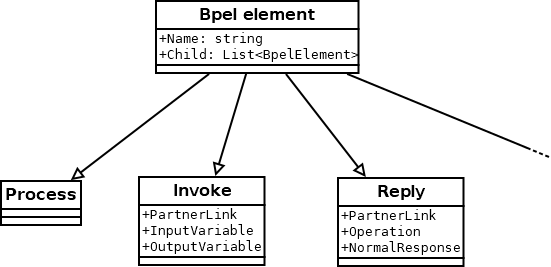
\includegraphics[scale=0.5]{images/BpelClass.png}
\caption{Az eddig leírt sablon}
\label{fig:bpelclass}
\end{figure}

\subsection{Petri háló}
A következő lépés a tervezetben, a "végtermék" leírása. Ahogy a BPEL-nél az volt szem előtt, hogy egy XML file miként dolgozható fel, és milyen elemekből áll, itt az lesz fókuszban, hogy a hálónak két típusa van, de mindkettő ugyan azon két főelemből épül fel, helyekből és tranziciókból. Alapvetően egy hasonló sablont kapunk itt is, amelyet a \ref{fig:petriclass}-es ábrán látunk.
\begin{figure}[h!]
\centering
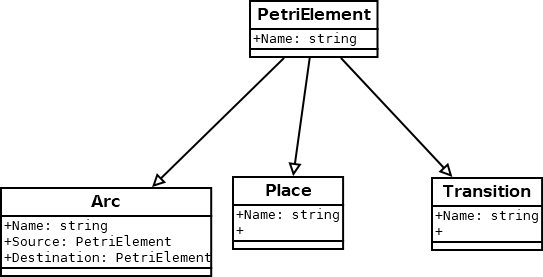
\includegraphics[scale=0.5]{images/petriClass.png}
\caption{A petri hálók prototípusa}
\label{fig:petriclass}
\end{figure}

Észrevehető, hogy a két ábra nagyon hasonló, de az elsőn jóval több leszármazott osztályt kellene feltüntetni. Észrevehető, hogy a diagram nem tartalmaz semmit, ami a színezett variánst megkülönböztetné. Ha megfigyeljük a színezett hálók leírását, rájövünk, hogy elég csak a hely és tranzició osztályt kibővíteni. Az így bővített osztályt a \ref{fig:colornet} ábra mutatja. Az élek gyakorlatilag csak a vizualizáció miatt szükségesek, ugyanis, az előbb említett osztályokat ha kiegészítjük \emph{mikor tüzelhet, milyen színnel, hová tüzelhet, stb. } paraméterekkel, akkor működésében a háló nem változik, de innentől a rajzolandó ábra nem tekinthető Petri-hálónak, hisz nincs benne él. Viszont az előbbi észrevétel hasznos a szimuláció és megjelenítés során, ugyanis nem történik mozgás az élen belül, csak a két végpontja között. 

\begin{figure}[h!]
\centering
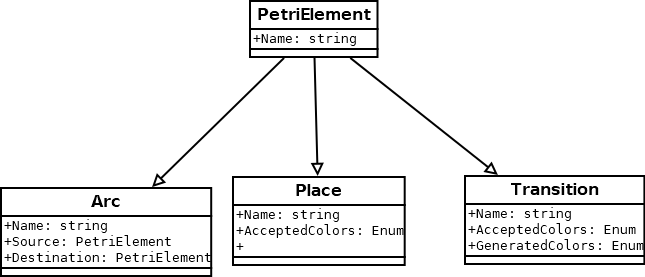
\includegraphics[scale=0.5]{images/PentC.png}
\caption{A színes háló}
\label{fig:colornet}
\end{figure}

Az így kapott ábra alapján már le tudjuk írni a színezett hálókat is. Észrevehetjük, hogy a helyek, az ábra szerint nem generálnak tokent. Viszont előfordulhat, hogy kezdéskor, vagy felhasználói bemenetre egy adott helyen jöhet létre token. Ez viszont nem mond ellent az ábrának, csak látszólag, ugyanis a helyek tényleg nem generálnak tokent, hanem inicializálva lesznek az adott mennyiségű tokennel, illetve felhasználói bevitel esetén a token a helyen megjelenik, kvázi mintha egy "rejtett" tranzició által kerülne oda a token. 

\Section{A vizualizáció megtervezése}
A vizualizáció gyakorlatilag két részből áll:
\begin{itemize}
\item a számítás eredményeinek listázásából,
\item a háló megjelenítéséből. 
\end{itemize}
Az eredmények listázása nem számít különösebben nagyobb feladatnak, ugyanis a kiíratást egyszerű szövegdobozok vagy label-ek elvégzik. Ami a vizualizációnál érdekesebb folyamat, az a háló generálása. 
A háló generálásánál, két opció adódik: az egyik, hogy sajt komponenst írunk a feladatra, a másik, hogy olyat használunk, ami már meg van írva és elérhető (lehetőleg szabadon). Utóbbi esetben szükséges egy olyan gráfleírónyelv használata, amit a program el tud fogadni. Az utóbbi opció sokkal logikusabb több indok miatt is:
\begin{itemize}
\item az open source szoftverek általában jól optimalizáltak,
\item kevés helyet foglalnak,
\item időt lehet vele megtakarítani, és
\item többnyire kielégítő dokumentációja van.
\end{itemize}

Innentől kezdve ha eldőlt a grafikus megjelenítés mikéntje, a következő lépés a hozzá szükséges gráf előállítása. Ez szintén két lépcsős folyamat. Először a forrásból kell petri-hálót generálni, majd a hálóból egy gráfleírónyelvi verziót. Ha tokenáramot szeretnénk rajta ábrázolni, akkor viszont olyan ábrát kell készíteni, ami könnyedén változtatható, és kellően látszik benne a tokenáram. A láthatóságot a gráfrajzoló legtöbbször önállóan vizsgálja, és úgy szerkeszti a gráfot, hogy az megfelelően olvasható legyen. A tokenáramot viszont kétféleképpen lehet ábrázolni: egy részeiben rajzolható aktív felületen, vagy egy teljesen passzív felületen, az egész kép cserélésével. Az első megoldás egy erre specializált architektúrát igényel, ami általában nem ingyenes, vagy nagyon sok módosítást igényel. A második módszer viszont szinte bárhol működik, cserébe a képét teljes egészében le kell generálni, így nagy háló esetén, illetve nagy számú tokenek esetén valószínűleg egy számításigényes időszakot kezd el. 

\Section{A leképzések megtervezése} 

A szoftver egyik fő komponense a converter. Ennek feladata a tényleges átalakítás előfeldolgozást követően.  A konverternek tudnia kell egy adott elemből egy az elemnek megfelelő részhálót előállítani. A konverzió során figyelni kell az eredeti elem tulajdonságait. A tulajdonságok után be kell állítani az új node típusát. Tranzició ugyanis működhet 'AND' és 'OR' módban is. Bár mindkettőre leggyakrabban binér műveletként tekintünk, a hálóban egy tranzició viszont nem feltétlenül csak kettő bejövő élt tartalmaz. A konverzió során ügyelni kell az eredeti elem tulajdonságaira, például mik az előfeltételek, vagy esetleg az aktivitás milyen további tokenmozgást indíthat el, és ennek hatására a háló további részein beállítani a megfelelő éleket. Ugyanakkor nem mindig képezhető le egy elem úgy, hogy megfelelően illeszkedjen a hálóra. A háló alapfeltétele ugyanis, hogy tranziciót csak hely követhet, és helyet is csak tranzició (élek közrefogásával).\\
A leképzés során használt forrás file viszont tartalmaz, a konverzió számára fölösleges XML nyelvi elemeket is. Például \texttt{porttype}, ami a folyamat külső eléréséhez szükséges. Az ilyen, és ehhez hasonló nyelvi elemek zöme azért elhanyagolható, mert a hálók csak helyre tudnak tokeneket fogadni külsőleg, és ameddig az meg nem történik a háló kvázi önszervező rendű.\\
Színes hálóknál viszont problémákba ütközünk. Az elsődleges probléma a színes tokenek. Az egyszerű háló csak egyféle tokent tud kezelni, emiatt lényegesen egyszerűbb a leképzése, de csak olyan folyamatokat enged leképezni, ahol a vezérjelet kell szimulálni. Tehát, ha vezérjel mellet megjelenik például egy függőség valamilyen külső objektumra, akkor a háló mindenképpen színes lesz (legalább kettő színnel). \\

\Section{Teljes terv}
Ha az eddig elkészült részegységeket összeillesztjük, egy elég jó alapvető képet kapunk a szükséges komponensekről. Ezt a \ref{fig:sysdes} ábra mutatja. Természetesen, mint minden rendszerterv ez sem tökéletes, hiszen legtöbbször implementáláskor történnek változtatások, általában az irányelvek betartása, valamilyen kényelmi szempont, vagy az előredefiniált implementálási módszerek hiánya miatt. Természetesen ilyenkor utólag az ábrát bővíteni szokás, de az már nem számít rendszertervnek, hanem a rendszer leírása mellett szokott helyet kapni. 
\begin{landscape}
\begin{figure}[h!]
\centering
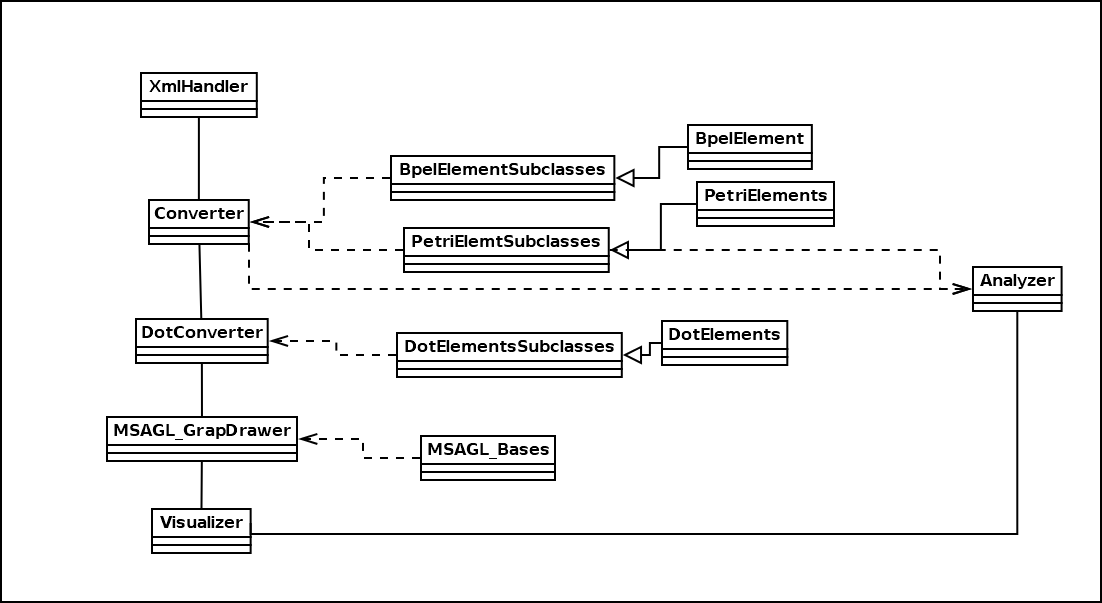
\includegraphics[scale=0.5]{images/sumdia.png}
\caption{Az összesített diagram}
\label{fig:sysdes}
\end{figure}
\end{landscape}
